\documentclass[11pt,a4paper]{article}
\usepackage[T1]{fontenc}
\usepackage{graphicx}
\usepackage{mathtools}
\usepackage{amssymb}
\usepackage{geometry}
\usepackage{titlesec}
\usepackage{enumitem} % 添加enumitem宏包
\usepackage{amsfonts}
\usepackage{amssymb}
\usepackage{fancyhdr} % 添加fancyhdr宏包
\usepackage{lastpage} % 添加lastpage宏包
\usepackage{graphicx} % 导入graphicx包
\usepackage{gensymb} % 引入gensymb包
\usepackage[UTF8]{ctex}
% 应用fancyhdr宏包的页脚样式
\pagestyle{fancy}
\fancyhf{} % 清除当前的页眉页脚设置
\fancyfoot[L]{免费开源,请勿商用} % 页脚左下方显示文字
\fancyfoot[R]{作者:阿尧} % 页脚右下方显示文字
\renewcommand{\headrulewidth}{0pt} % 去掉页眉的横线
\renewcommand{\footrulewidth}{1pt} % 设置页脚的横线宽度
\usepackage{draftwatermark} %增加水印
\SetWatermarkText{本真题由b站up陈瀚尧探索世界免费开源}
\SetWatermarkScale{0.3} % 可以调整为合适的大小
\SetWatermarkColor{gray!50} % 灰色透明度为50%

% 设置更窄的页面边距
\geometry{left=3cm, right=3cm, top=1cm, bottom=2cm}

% 设置section标题格式
\titleformat{\title}{\bfseries}{\thetitle}{1em}{}

% 设置section之间的距离
\titlespacing*{\section}{0pt}{3.25ex plus 1ex minus .2ex}{1.5ex plus .2ex}

\begin{document}
    \title{中国科学院大学\\2022年招收攻读硕士学位研究生入学统一考试试题\\科目名称:光学}
    \author{制作者:b站up 陈瀚尧探索世界}
    \date{}
    \maketitle
    % 设置section标题不显示序号
    \titleformat{\section}[block]{\normalfont\Large\bfseries}{}{0pt}{}

    % 设置itemize环境的项目符号为空
    \setlist[itemize]{label=} 

    \section{考试须知:}
    \begin{itemize}[topsep=0pt,itemsep=0pt,partopsep=0pt]
        \item 1.本试卷满分为150分,全部考试时间总计180分钟。
        \vspace{-3mm}
        \item 2.所有答案必须写在答题纸上,写在试题纸上或草稿纸上一律无效。
        \vspace{-3mm}
        \item 3.可以使用无字典存储或编程功能的电子计算器。(此条对于25考研可能作废)
    \end{itemize}
    \vspace{-5mm}
    \noindent\rule{\textwidth}{0.5pt} % 添加一条线
    \vspace{-12mm}
    \section*{一、填空题}
    \begin{enumerate}
        \vspace{0mm}
        \item 费马原理的内容是\underline{\makebox[4cm]{}}.
        \vspace{-3mm}
        \item 照相物镜相对孔径\underline{\makebox[2cm]{}}, 显微物镜数值孔径\underline{\makebox[2cm]{}}.
        \vspace{-3mm}
        \item 对正常人眼,观察$1m$目标,需调\underline{\makebox[2cm]{}}视度远点为$-0.2m$,近视镜\underline{\makebox[2cm]{}}度.
        \vspace{-3mm}
        \item $F=100mm$放大镜,其$p=$\underline{\makebox[2cm]{}},$2'$伽利略望远镜前加一个$f=100mm$正透镜,则组合放大率是\underline{\makebox[2cm]{}}倍.
        \vspace{-3mm}
        \item 白天人眼瞳孔$2.5mm$,夜晚$5mm$,光波长$550nm$,白天分辨角\underline{\makebox[2cm]{}},夜晚\underline{\makebox[2cm]{}}.
        \vspace{-3mm}
        \item 球差\underline{\makebox[4cm]{}},轴向色差\underline{\makebox[4cm]{}}.
        \vspace{-3mm}
    \end{enumerate}
    \section*{二、名词解释(共12分)}
    \begin{itemize}
        \item 1.光的反射;折射定律
        \vspace{10mm}
        \item 2.辐射通量;辐照度
        \vspace{10mm}
        \item 3.孔径光阑;视场光阑
        \vspace{10mm}
    \end{itemize}
    \section*{三、计算题:}
    \subsection*{3.直径$D=1m$的望远镜观察月球,能分辨月面上两点的最小距离?(地月距离$l=38\text{万千米}$,$\lambda =550nm$) (5分)}
    \vspace{10mm}
    \subsection*{4.正透镜$f=100mm$,小木棒$40mm$,平放在光轴上,木棒中点距凸透镜$200mm$.}
    \begin{itemize}
        \vspace{0mm}
        \item (1)木棒像的长短(6分)
        \vspace{0mm}
        \item (2)木棒绕中心90\degree时,木棒像的位置及大小(2分)
        \vspace{0mm}
        \item (3)物镜口径\(\mathcal{D}_{\text{物}}\)和目镜口经\(\mathcal{D}_{\text{目}}\) 
        \vspace{0mm}
        \item (4)出瞳距离\(\mathcal{L}_{z}\)
    \end{itemize}
    \vspace{20mm}
    \subsection*{5.显微镜$f_\text{物}=100mm$,$f_\text{目}=30mm$,两镜间隔$20mm$.(有可能数值是200),求:}
    \begin{itemize}
        \vspace{0mm}
        \item (1)显微镜视角放大率(2分)
        \vspace{0mm}
        \item (2)物体置于何处才能成像在目镜左方$250mm处$?问此时横向放大率?(6分)
        \vspace{0mm}
    \end{itemize}
    \vspace{20mm}
    \subsection*{6.$10^{x}$开普勒望远镜$f_\text{物}=100mm$,求目镜大小?(2分)与观察无限远目标相比,用此镜观察距离$500mm$处目标时,需调焦的距离为多少?若物镜与目镜间有足够多的调焦可能,问此时实际放大率为多少?(11分)}
    \vspace{10mm}
    \subsection*{7.简答题(每题4分 共12分)}
    \begin{itemize}
        \vspace{-3mm}
        \item (1)部分偏振光和椭圆偏振光是一回事吗?若是,给出理由;若不是,简单说明从实验上如何区分二者?
        \vspace{-3mm}
        \item (2)光在光纤中的传输原理基于什么光学现象?芯层$n=1.55$,包层$n=1.48$的光纤数值孔径是多少?
        \vspace{-3mm}
        \item (3)若使激光通过一个$n=1.76$的介质表面反射时无反射损失,对入射光有何要求?
    \end{itemize}
    \subsection*{8.一右旋圆偏振光,以45\degree由空气入射到玻璃界面$n_\text{玻}=1.55$,$n_\text{空}=1$,求反射率和反射光偏振状态(12分)}
    \vspace{15mm}
    \subsection*{9.杨氏双缝干涉,双缝相距$0.5mm$,双缝到屏距$1m$,点光源距双缝$30cm$,发射$\lambda =0.5\mu m$单色光.}
    \begin{itemize}
        \vspace{-3mm}
        \item (1)屏上与干涉条纹间距(6分)
        \vspace{-3mm}
        \item (2)若光源中心不变,但线宽增加$10nm$,求屏上干涉条纹消失的级次(6分)
    \end{itemize}
    \vspace{15mm}
    \subsection*{10.在光学玻璃基片($n_G=1.5$),在其上面镀了一层氟化镁膜层($n_\text{氟化镁}=1.38$,入射$\lambda =0.5\mu m$),求正入射时给出的最大反射率和最小反射率的膜厚度及相应的反射率.(12分)}
    \vspace{15mm}
    \subsection*{11.天文望远镜直径为$D=100mm$,人眼瞳孔直径$d=2mm$求对于发射波长$\lambda =0.5\mu m$光的物体角分辨极限,充分利用物镜分辨本领,该望远镜的放大率$M$应选多大为宜?(12分)}
    \vspace{15mm}
    \subsection*{12.缝宽$a=0.09mm$,双缝间隔$d=0.7mm$,照明波长$\lambda =0.632.8\mu m$的双缝衍射,问在中央极大值两侧的两个衍射极小值间,将出现多少个干涉极小值,若屏离开双缝$2m$时计算其余纹宽度(14分)}
    \vspace{15mm}
    \subsection*{13.方解石制成两个带有空气间隔的偏振棱镜,其中棱镜1的光轴垂直于入射面,光线按图示方向入射,已知$n_o=1.658$,$n_e=1.486$。}
    \begin{itemize}
        \vspace{-3mm}
        \item (1) 求$\alpha $角在大于多少范围内,才能使入射的自然光经过棱镜后变为线偏振光。(4分)
        \vspace{-3mm}
        \item (2)若入射光强度相同,哪个棱镜的出射线偏振光更强?(4分)
        \vspace{-3mm}
        \item (3)画出自然光入射时的传输光路以及光的偏振状态。(6分)
    \end{itemize}
    \vspace{-3mm}
    % 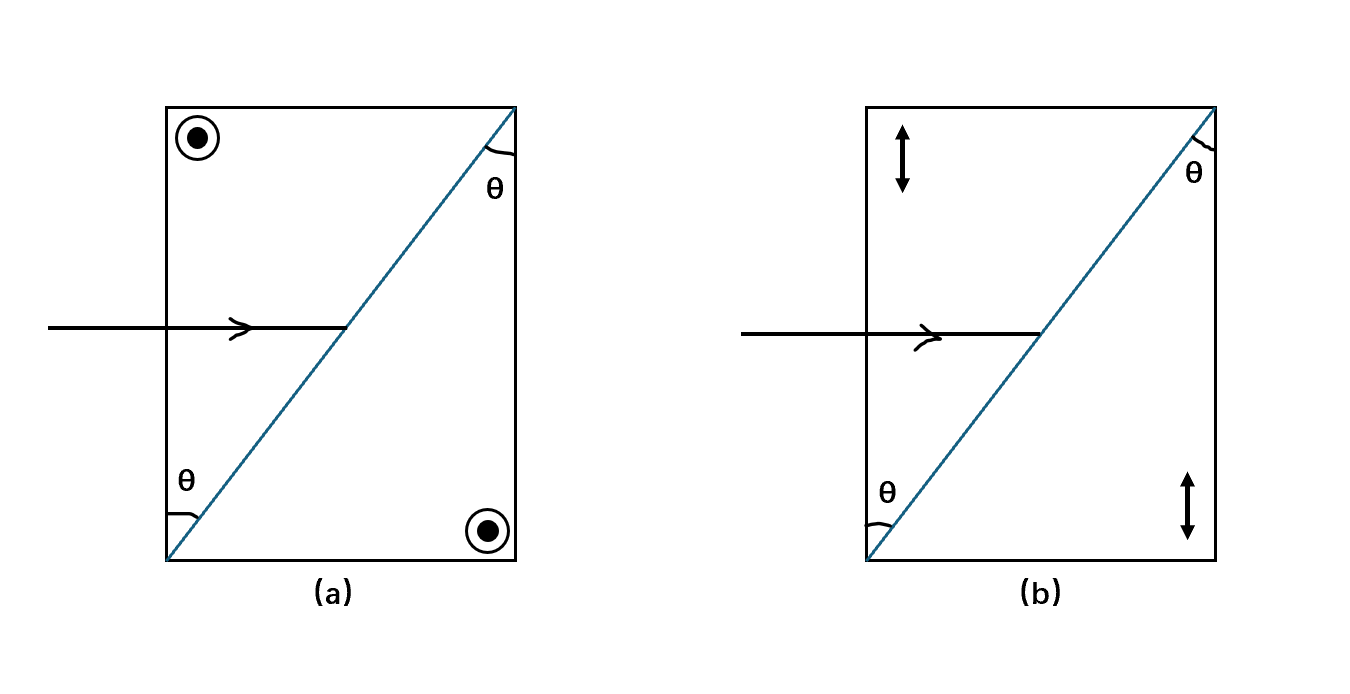
\includegraphics[scale=0.2]{7.png}% 插入图片,按50%的比例缩放
    \subsection*{14.KDP晶体:$L=3cm$,$d=1cm$,$\lambda =0.5\mu m$时,$n_o=1.51$,$n_e=1.47$,$V_\text{半波}=10.5x10^{-2} \frac{m}{V}$(共12分)}
    \begin{itemize}
        \vspace{-3mm}
        \item (1)纵向运用相位延迟为$\varphi = \frac{\pi}{2}时,外加电压为多少?$
        \vspace{-3mm}
        \item (2)此电压下,一束振动方向与其感应折射率全轴x轴成45\degree的线偏光的出射后偏振态。
    \end{itemize}
    \vspace{-3mm}
\end{document}